\autsection{Radiation Protection during EDL}{Maja Tomicic}\label{chap:radedl}

As described in chapter \ref{sec:radiation_environment} the radiation environment around and on the surface of Europa is extremely harsh and expansive radiation protection is needed to ensure the reliability and safety of critical systems and subsystems within the payload. Thus the protection of the payload from the radiation during the landing is an important design driver. The need for radiation shielding is conflicting with the severe mass and volume limitations of the lander, and novel and creative designs are necessary to accommodate both issues.

\subsection{Material}

When choosing the material for the tank structure the most important factors are strength, radiation shielding properties, mass and experience from previous missions ensuring durability and reliability under temperature fluctuation and in vacuum. 

Aluminum has always been the material of choice for space structures of all types. Its light weight, strength, ability to withstand stresses due to temperature fluctuations during operation in space, and its durability over long periods of time, has made aluminum very popular for space applications. However Aluminum does not have good shielding effectiveness relative to its mass, and therefore composite materials have been considered for this mission.\\

\noindent
Advanced fiber-reinforced poly-ethene materials have shown significant property advantages that make them excellent candidates for use in spacecraft structures. Properties such as specific tensile strength, specific tensile modulus, fatigue resistance, damage tolerance, and design flexibility all make these materials very attractive. Additionally, the composite materials are much better radiations shields against GCR and solar flares than metals such as aluminum or titanium. The advantage of plastic-like materials is that they produce far less "secondary radiation" than heavier materials like aluminum. A specific polyethylene composite material RXF1, invented by NASA, is stronger than aluminum (3 times the tensile strength) and lighter than aluminum (2.6 times lighter), is 50$\%$ better at shielding solar flares and 15$\%$ better at shielding cosmic rays \cite{RXF1}.However the polymer-based composites are not as resilient to thermal fluctuations without significant modification to their chemical structure and have shown to be flammable. As a result, polyethylene-based composites without thermal shields will have to support the structure (in addition to providing radiation shielding) from within the interior of the pressure vessel or from within a cavity between two metallic walls. Also, these materials are susceptible to environmental degradation in vacuum. \\
 
\noindent
Radiation protection and mass, are both driving and constraining factors. Despite showing great qualities that surpass that of aluminum in both those factors, the poly-ethene based materials are not chosen for the tank material, due to the uncertainties in their response to thermal fluctuations and other environental conditions that the landing module will experience during the long deep-space journey and the EDL. \\

\noindent
Because of their shielding and mechanical properties, polymer-based composites
are expected to make up a good part of the internal structure of the future space vehicle designed for
extended deep-space missions  \cite{rad_shield_2006}. And future work could asses the possibility of graded tank walls of alternately aluminum and poly-ethene composite. 


\subsection{Radiation protection design}
To achieve the most mass efficient radiation shielding the payload is surrounded by a toroidal fuel tank. This design provides radiation shielding as a combination of shielding from the liquid propellant surrounding the payload and shielding by the tank aluminum walls. For mass considerations the inner wall surrounding the payload, which most efficiently protects the payload, is thicker (7 mm) than the larger outer wall (2 mm). The design is illustrated in figure \ref{fig:tankdesign}.

\begin{figure}[htb]
\begin{center}
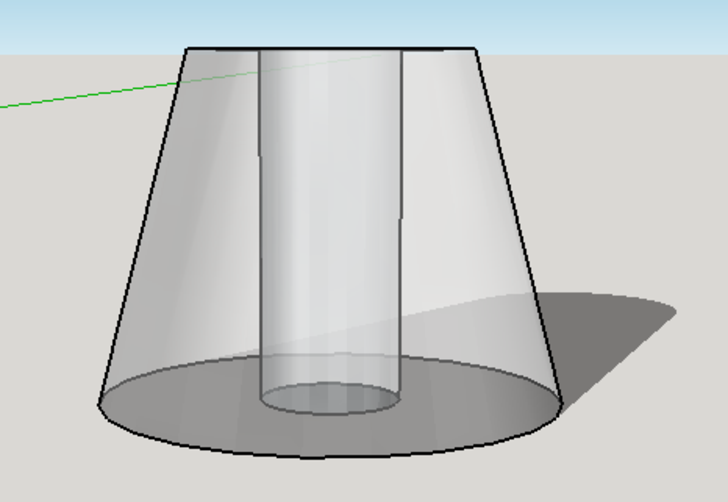
\includegraphics[scale=0.7]{figures/navtheory/tank}
\caption{Sketch of the tank design. The payload will be placed in the cylinder-shaped hole, thus being protected from the radiation by a combination of the liquid propellant and the aluminum walls of the tank. The inner wall surrounding the cylinder is thicker (7 mm) compared to the outer tank wall (2 mm). }
\label{fig:tankdesign}
\end{center}
\end{figure}

The main propellant stored in the tank will be liquid hydrazine (N$_2$H$_4$). Materials rich in hydrogen and carbon are known to be effective shielding materials against energy radiation because they do not fragment into secondary particles as much as heavier elements when bombarded by high-energy radiation \cite{rad_shield_2006}. Thus the hydrazine will be an excellent radiation shield. 
However, the propellant will be consumed during the landing, thus not being efficient during the final part of the landing. Therefore the final radiation dose has been calculated as a worst case scenario where only the tank walls are considered. \\

\noindent
Figure \ref{fig:raddose} shows the 2$\pi$ radiation dose in Rad/hour on the surface of Europa as a function of aluminum shielding thickness. From it, it is seen that with a shielding of 9 mm of aluminum the received 2$\pi$ dose would be $\sim$250 Rad/hour. This amounts to a 4$\pi$ dose of $\sim$100 Rad during the landing and the 250 Rad/hour after landing on the surface.

\begin{figure}[htb]
\begin{center}
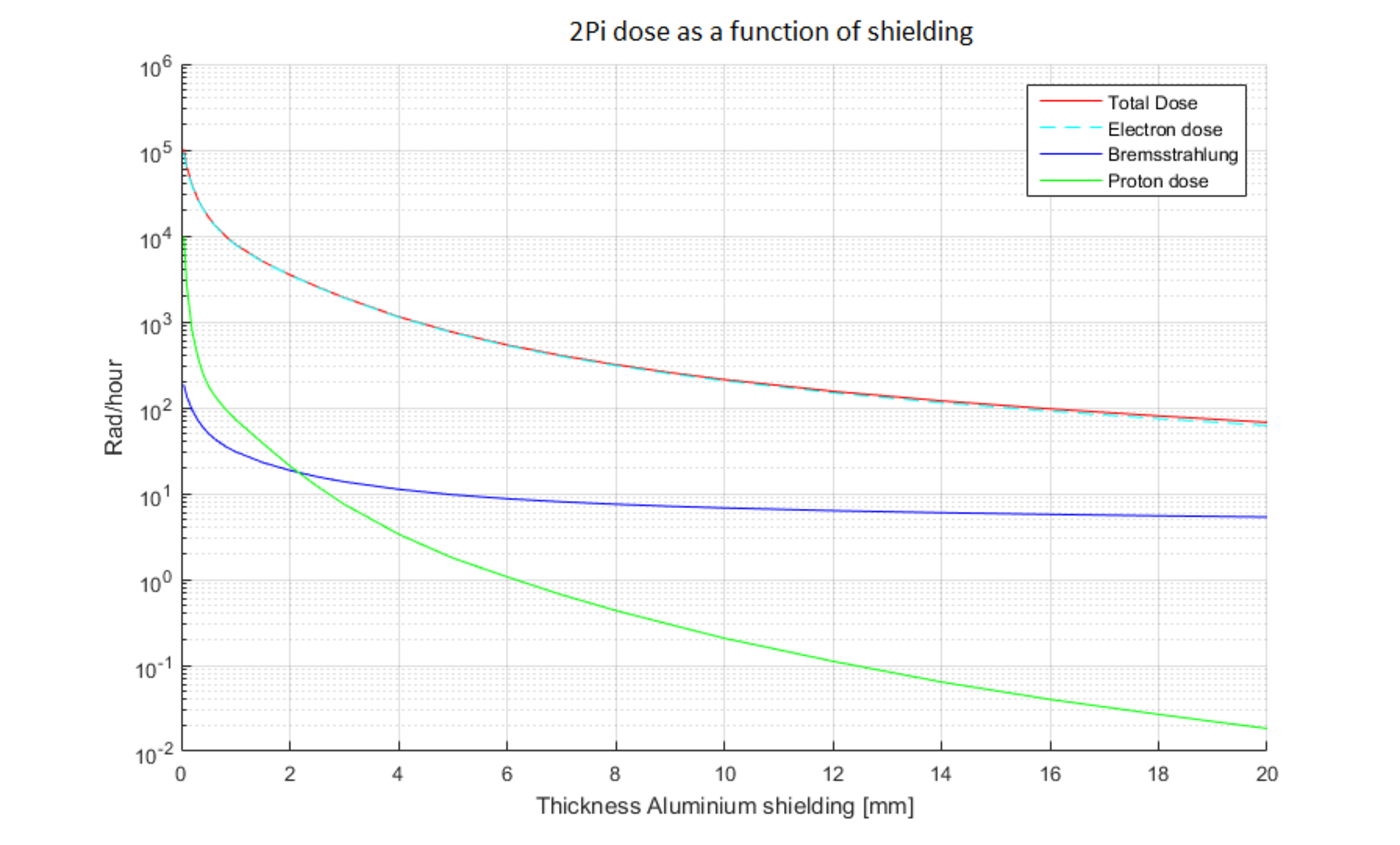
\includegraphics[scale=0.48]{figures/navtheory/dose}
\caption{Dose received on Europa in Rad/hour as a function of aluminum shield thickness. The graph is made with data from SPENVIS.}
\label{fig:raddose}
\end{center}
\end{figure}
